\section{Conceptual design options} \label{ch:options}
This chapter will discuss the five design concepts which will be considered in this report. First of the selection of the concepts based in the shape, mission duration and controls system design option trees is considered. Finally in Section \ref{sec:conf} the five selected configurations are sketched. 

\subsection{Concept section}
 From the \acrfull{br} three deign options three were made for the design of the decelerator. In these design consideration the shape, mission duration and control system are considered. This yielded a set of all the individual design considerations separately. The design options are shown in Figure \ref{fig:dotshape} to \ref{fig:dotcontrol}. From these design option trees a feasible set of design option can be considered. From Figure \ref{fig:dotshape} showing the design option six shapes can be considered. This can consequently be combined with three possible control systems from Figure \ref{fig:dotcontrol}. The mission duration in is integral to any design chosen. It is therefore considered in any mission. 

\begin{figure}[H]
%\centering
\hspace{-23mm}
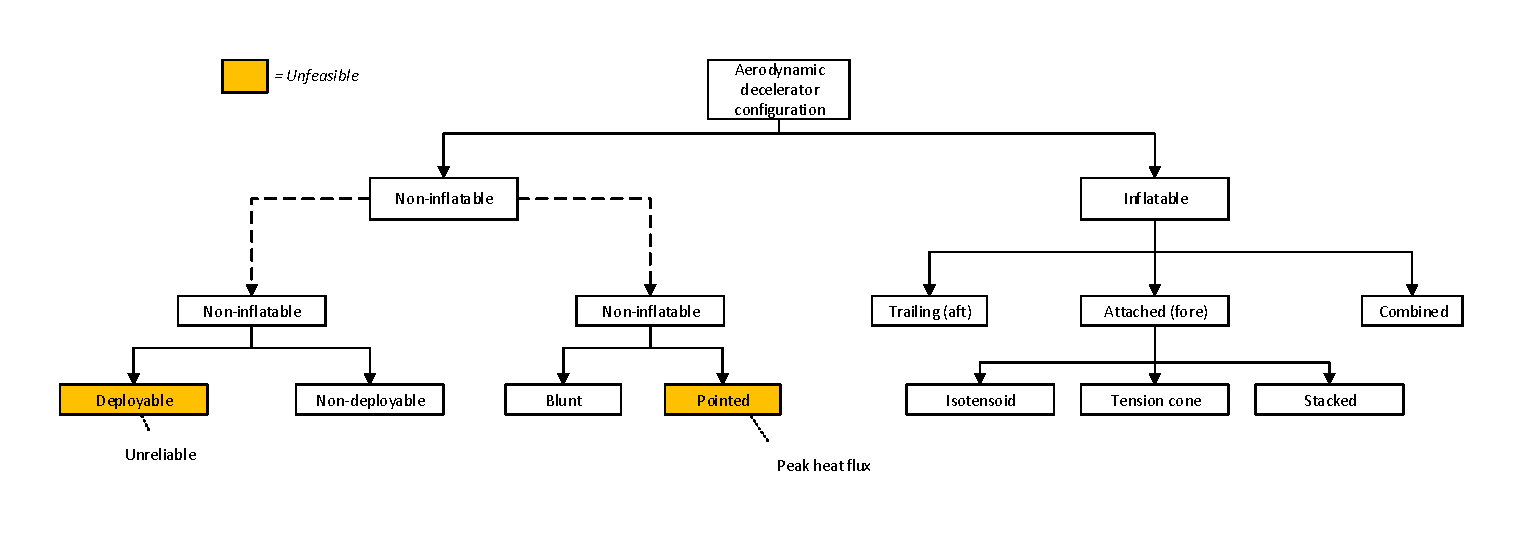
\includegraphics[width = 1.25\textwidth]{Figure/DOT_configuration.pdf}
\vspace{-5mm}
\caption{Design Option Tree for entry vehicle configuration}
\label{fig:dotshape}
\end{figure}

\begin{figure}[H]
\centering
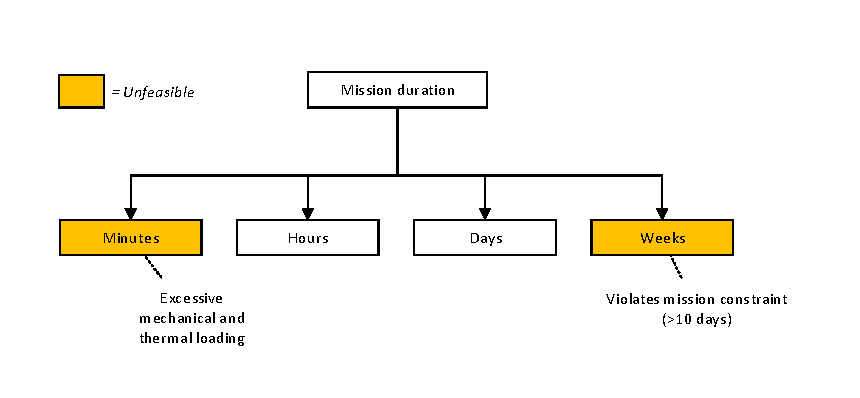
\includegraphics[width = 1.0\textwidth]{Figure/DOT_missionduration.pdf}
\vspace{-5mm}
\caption{Design Option Tree for mission duration}
\label{fig:dotduration}
\end{figure}

\begin{figure}[H]
\centering
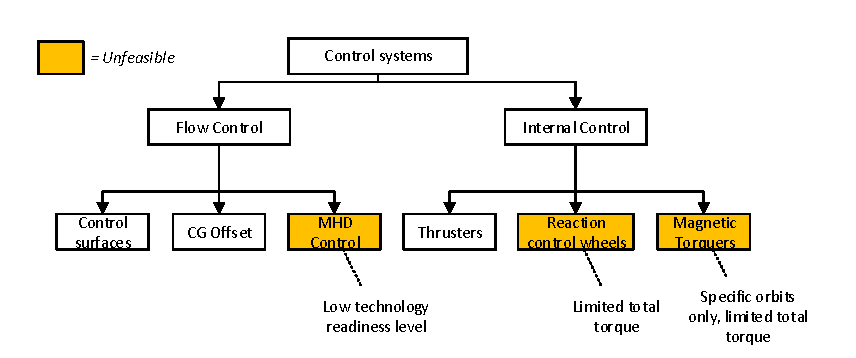
\includegraphics[width = 0.93\textwidth]{Figure/DOT_control.pdf}
\vspace{-5mm}
\caption{Design Option Tree for control systems}
\label{fig:dotcontrol}
\end{figure}


From the above discussed 18 options of shapes and control systems some me be disregarded immediately since they cannot be combined. From this point onwards the shape will be considered leading. The control systems from Figure \ref{fig:dotcontrol} are considered separately for each possible state for each defined shape. Design option trees were only made for the shape and controls surface as these require individual matching as not any shape and control surface may be combined. Analysis on the performance in the field of aerodynamics, thermodynamics or structures follow directly from the shape. The control surface is however considered separately and exotic concepts such as the, for now, deemed infeasible \gls{mhd} control have their own strict requirements on the structure. Since these exotic options are at this point deemed infeasible the shape of the structure can be considered leading in the design. 

 Table \ref{tab:designconcepts} shows the design option that will be considered within this report. The check-marked control systems are further investigated for their feasibility and performance within ?? the chapter discussing the control systems. For these control systems their performance need to be considered separately and their feasibility must be properly supported by either references or computations. The use of a \gls{cg} offset as a control mechanism may for example be doubtful since the demonstration on its performance is only done in the \gls{irve} in which the \gls{hiad} has a relatively high mass fraction compared to the payload \cite{Dillman2012}. For this design from the requirement CIA-Op-A02-02 (Appendix \ref{app:req}) this mass fraction is however specified to be only 10\% doubting the effectiveness of a \gls{cg} offset as control system. For control surfaces only specific designs may be possible resulting in only the use of for example body flaps or morphing the inflatable as control mechanism. All these considerations are again discussed in Chapter ... . These results are finally used as one of the selection criteria in the trade off.

It must again be noted that the control configurations of Table \ref{tab:designconcepts} feature the primary control mechanism. These may always be appended later on in the design process, after the trade-off, if additional control systems increase the overall performance. 

\begin{table}[H]
	\caption{Generation of design concepts}
	\label{tab:designconcepts}
		\begin{tabular}{|p{0.3\textwidth}|p{0.22\textwidth}|p{0.22\textwidth}|p{0.22\textwidth}|} \hline 
			\textbf{Concept} & \textbf{Thruster}	& \textbf{\gls{cg} offset} &  \textbf{Control surfaces} \\ \hline \hline
			Stacked toroid   & \cmark	& \cmark &  \cmark \\ \hline
			Iso tensoid		 & \cmark	& \cmark &  \xmark\\ \hline
			Tension cone	 & \cmark	& \cmark &  \cmark \\ \hline
			Trailing 		 & \xmark	& \cmark &  \cmark \\ \hline
			Combined 		 & \xmark	& \cmark &  \cmark \\ \hline
			Rigid  		   	 & \cmark	& \cmark &  \cmark \\ \hline
		\end{tabular}
\end{table}

At this point it may be noted that at this point in Table \ref{tab:designconcepts} for each shape a possible control mechanism can be considered. Rather just three combinations are deemed infeasible. Thrusters are not considered for the Trailing an Combined configuration. Due to the aft elements of these designs thruster cannot be considered the primary control mechanism. Due to the large moments of inertia (due to aft elements) and very high stability of the aft systems (e.g. compare to a parachute) thrusters cannot be considered due their inefficiency. 

For the Iso tensoid configuration controls surface are not deemed possible since the whole outer surface is covered by the inflatable. Controls systems such as for example body flaps cannot therefore not be placed. Using morphing of the structure as control surface is also considered unfeasable since again the whole outer surface is covered. 

Finally, although not deemed infeasible from Table \ref{tab:designconcepts}, the Combined concept is disregarded. It is considered to be too similar to a Trailing concept. A trailing concept will still require a heat shield at the front of the payload and can therefore be considered, is some aspects, a Combined configuration as well. It is therefore considered that a deployable inflatable at the front will have no additional advantage. A small deployable will have a similar performance as the Trailing configuration, but features the additional complexity of the front inflation system. A large frontal inflation systems will however place the aft inflatable in the wake making it effectively useless. Removing the aft declarator will however yield a "simple" Stacked toroid, Iso tensoid or tension cone configuration. For these reasons the Trailing concept will not be considered. 


...Control department moet het hier mee eens zijn. Hier kunnen nog combinaties weg gehaald worden en naar het control chapter verplaatst worden (of andersom)... 

..Check of alle argumentatie zoals besporeken er in zit... Uiteindelijk te weing argumentatie --> Naar control chapter

\subsection{Concept configurations} \label{sec:conf}

In this section a the global configuration of each of the final five shapes is considered. Figure ...